%%%----------------------------------------------------------
\chapter{Aims and Context}
%%%----------------------------------------------------------
\section{Introduction}\label{sec:introduction}
% describe problem
The aim of this project is the implementation of the article \textit{"Consistent Depth Maps Recovery from a Video Sequence"} \cite{Zhang2009}, by Zhang, Jia, Wong, and Bao and published in \textit{Transaction on Pattern Analysis and Machine Intelligence} (TPAMI).
%The article describes an algorithm which is able to generate a sequence of \emph{depth-maps} starting from an RGB-video.
The problem faced by Zhang et al. consists in estimating the {depth-maps}\footnote{A \emph{depth-map} is an image in which each pixel maintains depth information.} for all the frames contained in source RGB-video of a static scene.
More precisely, given an image sequence, the aim of the paper is to estimate a sequence of depth-maps having temporally consistent depth values.
This depth-maps can then be  used in several different of tasks; scene reconstruction and layer separation are two such examples. Having the depth values for all images in a video could also allow the usage of more sophisticated image processing techniques, an example could be the addition of virtual shadows in the source video.
\begin{figure}[!h]
	\centering
	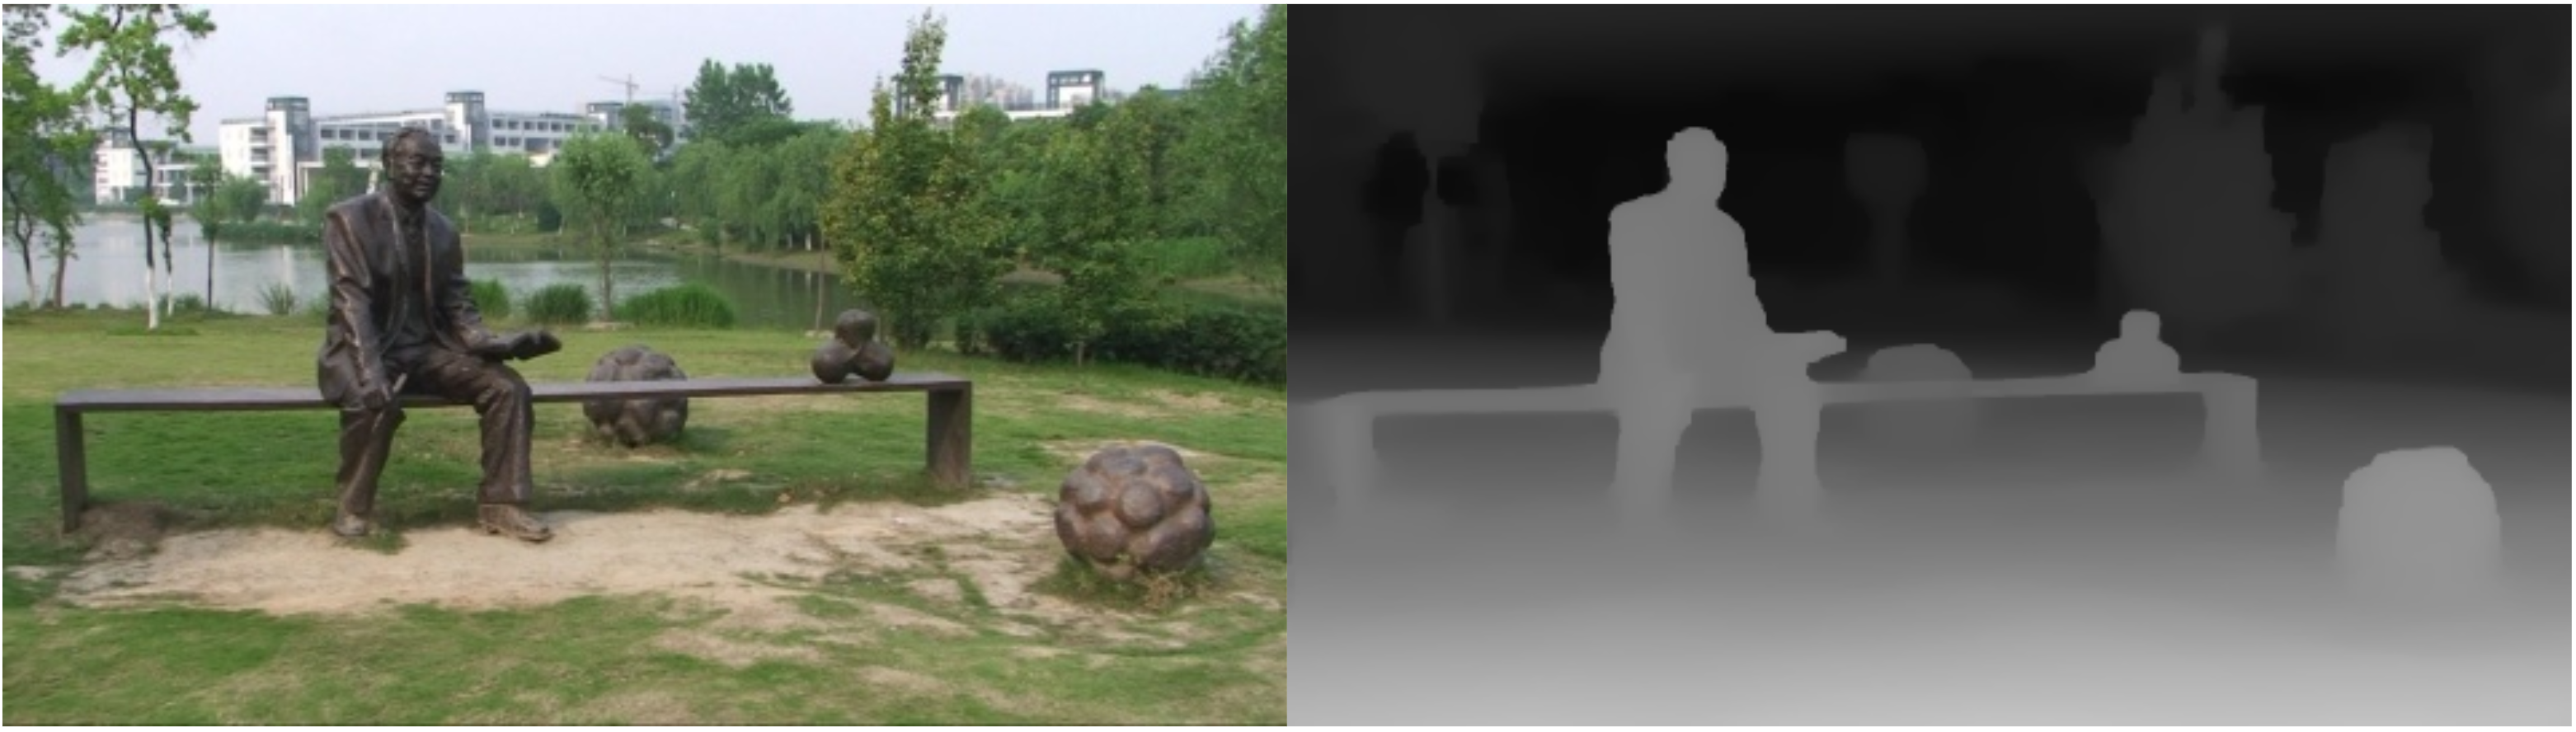
\includegraphics[width=.95\textwidth]{depthmap_example.png} %{CS0031}
	\caption{One of the estimated depth-maps  obtained using the approach described in \cite{Zhang2009} over a sequence of 200 images.}
\end{figure}
% TODO no explicit modeling of occlusion and noise
% TODO robust against noise
%One interesting feature of the approach in \cite{Zhang2009}
\begin{tcolorbox}[title=Note:]
While a free-of-charge implementation is available on the authors' website (\url{www.zjucvg.net}), they do not offer its source code; hence, the reasons behind this project are to offer an open-source implementation of said article, and to offer didactic improvement for the project's author.
This report's implementation can be found in the \Github{} repository
\ProjectUrl{}.
\end{tcolorbox}
%\footnote{See  Zhejiang University's {Computer Vision Group} website: \url{www.zjucvg.net}}

\section{Proposed Approach}
% overview of proposed solution
The approach proposed in the original article consists of four steps:
\begin{description}
\item\textbf{Camera Parameters Estimation.} During this phase, the camera parameters (\ie \emph{position}, \emph{rotation}, and \emph{intrinsic matrix}) are estimated using a \emph{Structure From Motion} (\SFM) algorithm. Unsurprisingly, the one used in the article is also related to a previous publication (see \cite{Zhang2007}) done by Zhang and Bao in collaboration with another research group. It is worth to note that \SFM{} algorithms can also produce as output a sparse cloud of 3D feature points (the ones used for the calibration). This is important since these points are also utilized during the depth-maps recovery. 
\begin{figure}[!h]
	\centering
	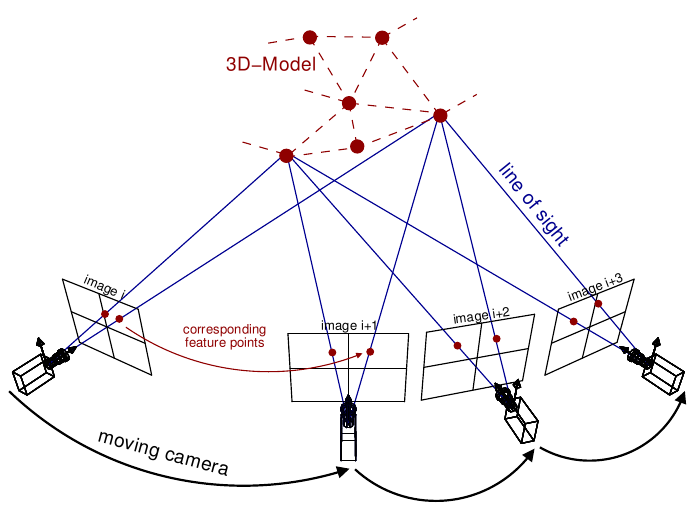
\includegraphics[width=.5\textwidth]{sfm.png} %{CS0031}
	\caption{SFM photo-grammetric approach; it tracks features points over different frames in order to infer the camera parameters. Source: \url{Theia-sfm.org}}
\end{figure}


\item\textbf{Disparity initialization.} 
For each frame in the video, a raw estimation of the corresponding depth-map is computed; this is achieved by minimizing an energy function whose parameters are the depth values to estimate.
These raw depth-maps are successively processed using a plane fitting algorithm: each image is divided into segments using \emph{mean-shift color segmentation} \cite{Comaniciu202}, these segments are then considered as a set of planes and fitted to the existing depth-maps raw values. The resulting images are the initialized depth-maps, ready to be used in the next step.

\item\textbf{Bundle Optimization.} The depth-maps obtained during the initialization process are then refined by applying geometric coherence constraints. This refinement process iteratively elaborates the given raw data by minimizing an energy function similar to the one used in the previous step, but enriched with geometric-consistency constraints.

\item\textbf{Space-Time Fusion.} This is the final step of the process, and it is used to polish the results obtained from the previous steps and removing eventual remaining noise.
The estimated depth-map values are used to define a loss function  that can subsequently be optimized through the use of iterative \emph{Conjugate Gradient Method}, an optimization technique able to find approximate solution to energy-minimization  problems.
The designed loss function takes into consideration: \emph{spatial continuity} between already computed depth-values, \emph{temporal coherence} of the estimated depth-maps, and consistency with the sparse points obtained by the \SFM{} algorithm used to compute the camera parameters.
\end{description}
 

%\section{Related Work}
%Since the proposed approach makes use of a variety of techniques, and it is relatively old (2009), the related work section is organized as follows:



